\subsection{Numerical results}
We used equation \eqref{e9} to obtain first non-stationary numerical result using \texttt{Octave} function \texttt{ode45}, that solve equation with the well known explicit Runge–Kutta method of order (4,5).  The point here was to make a first step to a better understanding of the roles of the different parameters of our equation that seem of interest to us, \textit{i.e.} the resistance $R$ and the permeability $L_p$. We also aim at comparing the behaviour of IOP on different patient profile. 

For sake of simplicity we focus on patient arterial pressure. We consider three arterial pressure profiles : a low arterial blood pressure  (LBP) of $26.6$, a normal arterial blood pressure (NBP) of $31.1$, and a high blood arterial pressure (HBP) of $35.5$.

We take physiological datas from the literature \cite{lyubimov2007,anders1975,To2002 }, and our initial values in physiological range. As it is a first step forward such simulations, we decide to neglect here the oscillating component. 

The first simulation we perform is a long time scale simulation. We compute the equation \eqref{e9} and look at the results for IOP and $C_2$ over time for our three arterial profile patients. The results of this simulation are plotted fig.~\ref{fig:tevolpc2}.

\begin{figure}[htbp]
 \centering
  \subfigure[Time evolution of IOP\label{fig:IOPt}]{
    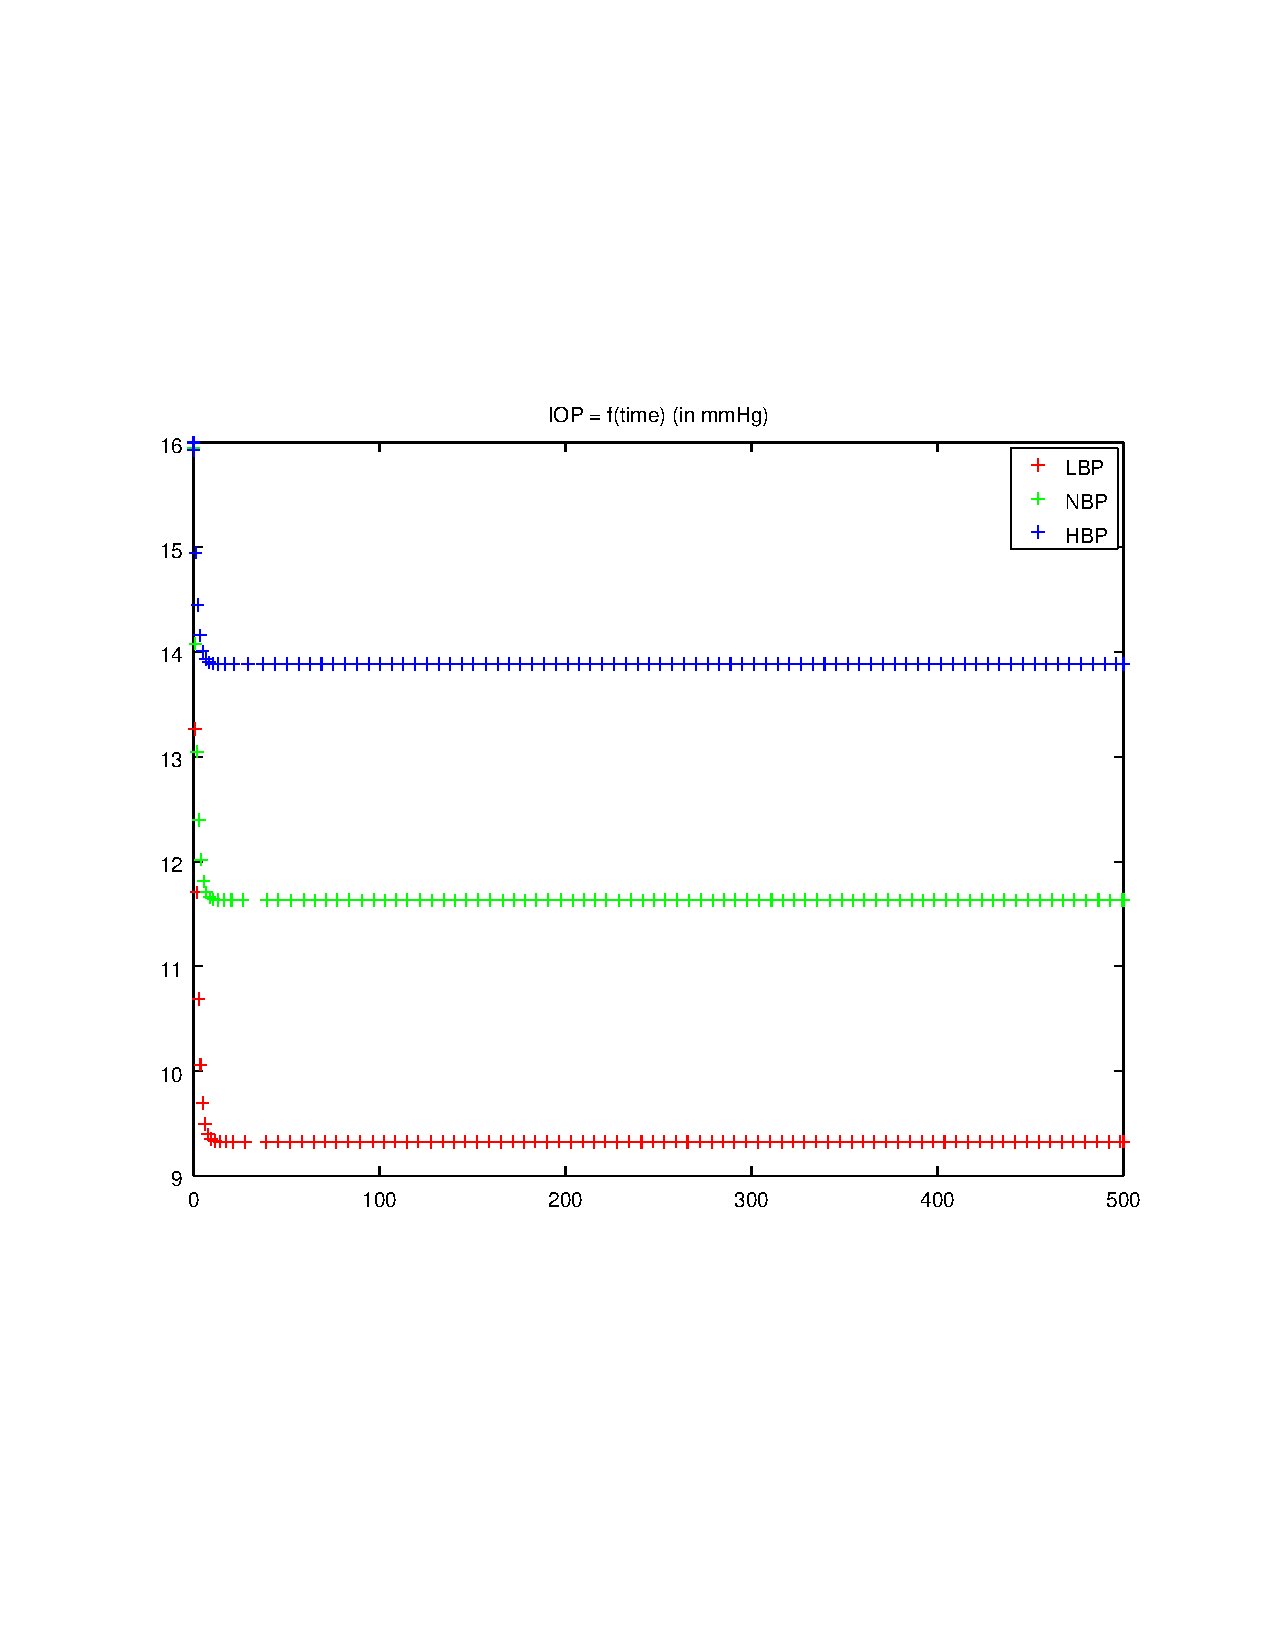
\includegraphics[width=0.55\textwidth]{images/IOP_time}
  }
  \subfigure[Time evolution of $C_2$\label{fig:C2t}]{
   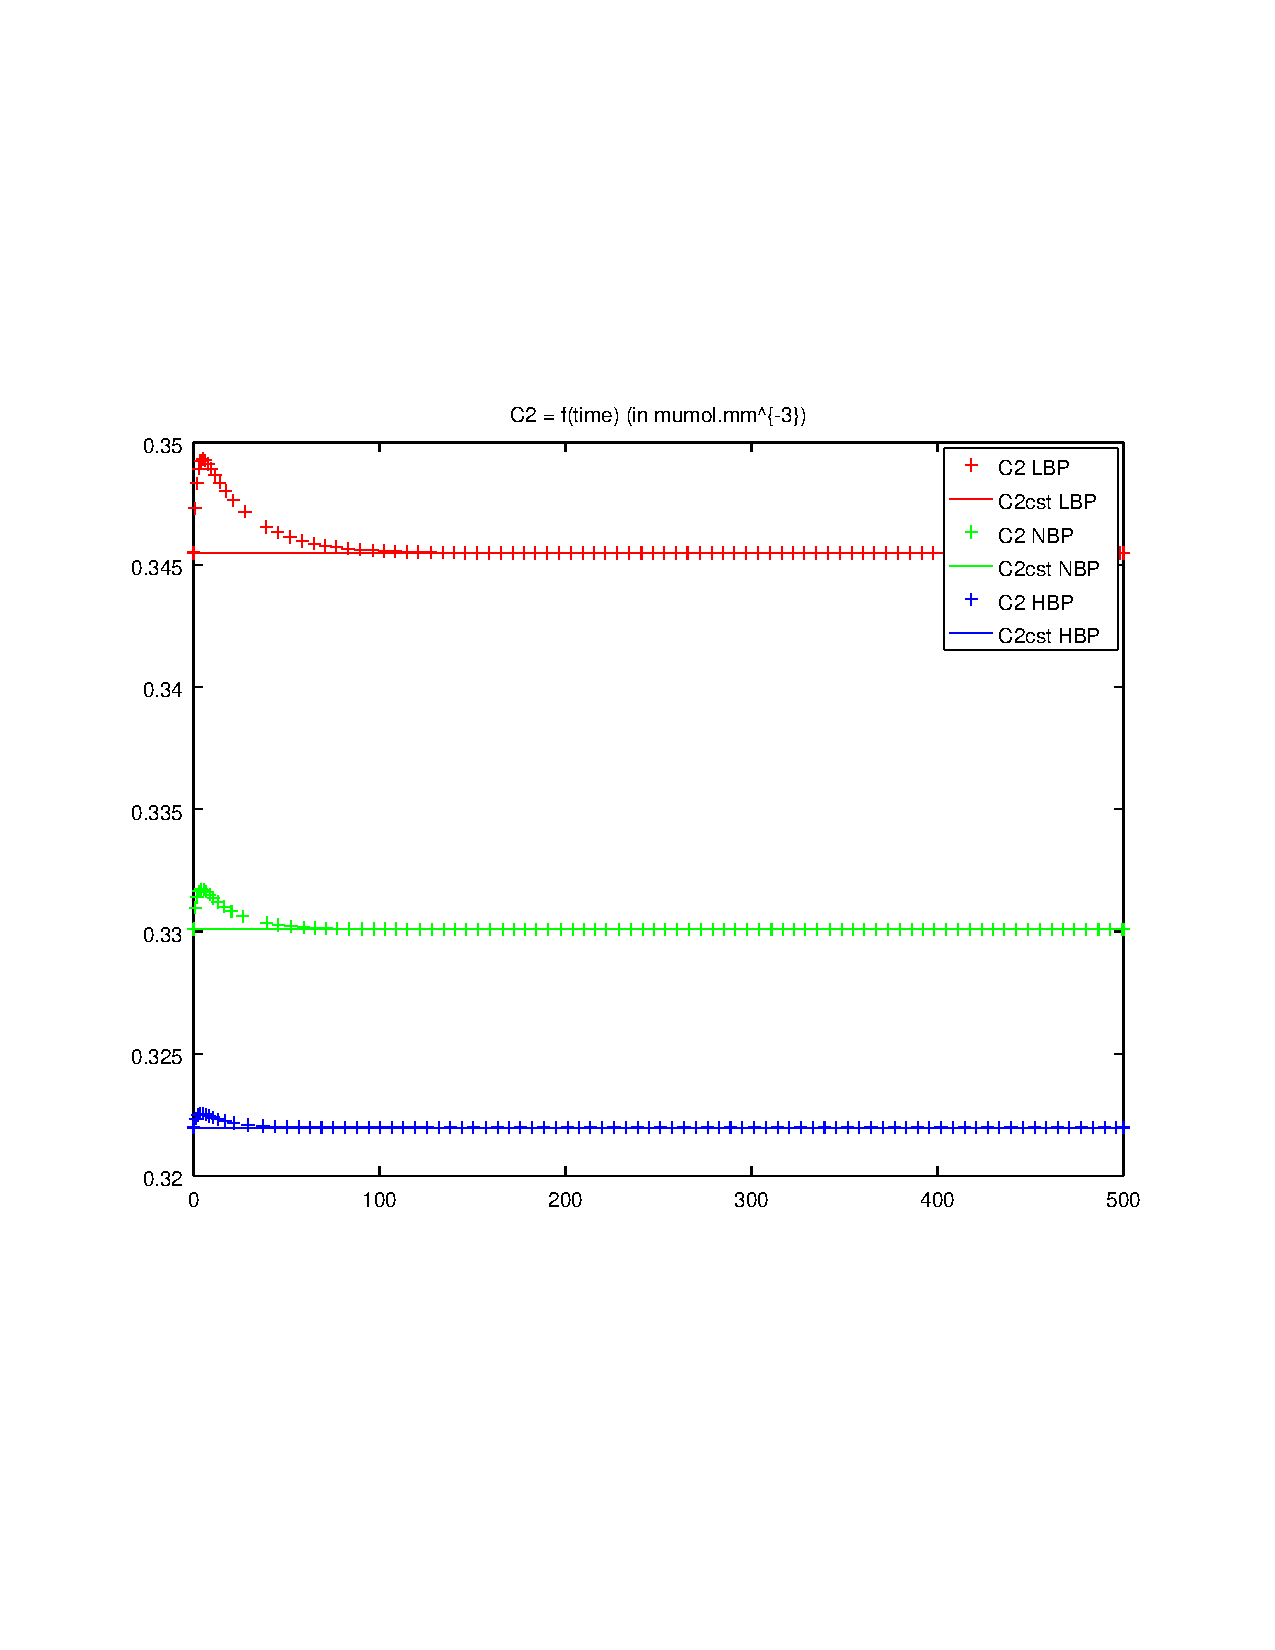
\includegraphics[width=0.55\textwidth]{images/C2_time}
 }
 
  \caption[text1]{Time evolution of IOP and $C_2$ }
    \label{fig:tevolpc2}
\end{figure}
The simulation clearly points out the different behaviour regarding the arterial pressure. The IOP seems to decrease widely more for a low $p_a$. This seem to be relevant from a physiological point of view. For more clarity we represented IOP and $C_2$ at a final time as histogram in fig.~\ref{fig:histc2} and~\ref{fig:histIOP}. The histogram visualisation helps us understand the different reactions of IOP and $C_2$ on different $p_a$. Again we can see than HBP patients tend to have a higher $IOP$ but a small low component concentration than patients with lower blood pressure.
\begin{figure}[h]


\begin{center}
  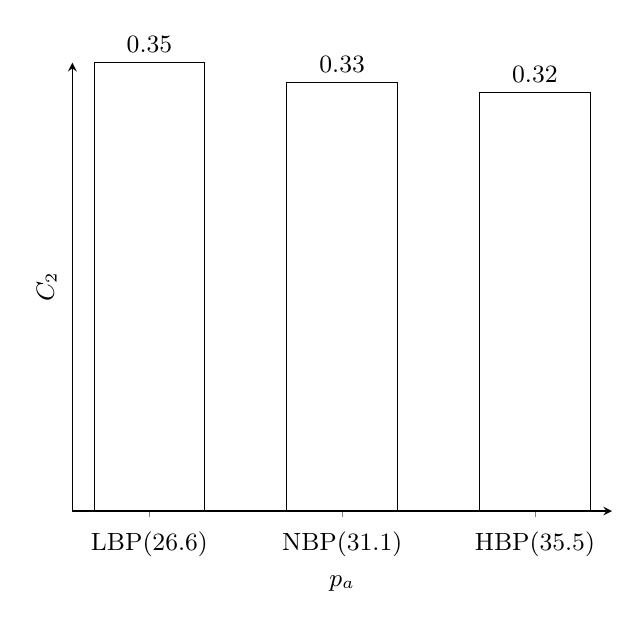
\begin{tikzpicture}[font=\small]
    \begin{axis}[
      ybar,
      bar width=40pt,
      xlabel={$p_a$},
      ylabel={$C_2$},
      ymin=0,
      ytick=\empty,
      xtick=data,
      axis x line=bottom,
      axis y line=left,
      enlarge x limits=0.2,
      %symbolic x coords={excellent,good,average,bad,awful},
      symbolic x coords = {LBP(26.6),NBP(31.1),HBP(35.5)},
      xticklabel style={anchor=base,yshift=-\baselineskip},
      nodes near coords={\pgfmathprintnumber\pgfplotspointmeta}
    ]
      \addplot[fill=white] coordinates {
        (LBP(26.6),0.345)
        (NBP(31.1),0.330)
        (HBP(35.5),0.322)
      };
    \end{axis}
  \end{tikzpicture}
  \end{center}

  \caption{$C_2 = f(p_a)$}
  \label{fig:histc2}
\end{figure}
\begin{figure}[h]
\begin{center}
  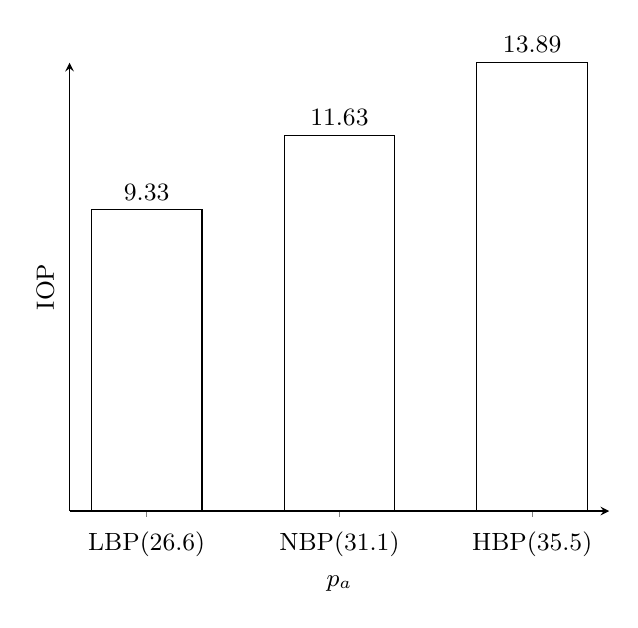
\begin{tikzpicture}[font=\small]
    \begin{axis}[
      ybar,
      bar width=40pt,
      xlabel={$p_a$},
      ylabel={IOP},
      ymin=0,
      ytick=\empty,
      xtick=data,
      axis x line=bottom,
      axis y line=left,
      enlarge x limits=0.2,
      %symbolic x coords={excellent,good,average,bad,awful},
      symbolic x coords = {LBP(26.6),NBP(31.1),HBP(35.5)},
      xticklabel style={anchor=base,yshift=-\baselineskip},
      nodes near coords={\pgfmathprintnumber\pgfplotspointmeta}
    ]
      \addplot[fill=white] coordinates {
        (LBP(26.6),9.3270)
        (NBP(31.1),11.632)
        (HBP(35.5),13.886)
      };
    \end{axis}
  \end{tikzpicture}
  \end{center}

  \caption{$IOP = f(p_a)$}
  \label{fig:histIOP}
\end{figure}

%\begin{figure}[h]
%\begin{tabular}{|l|l|l|l|}
%\hline
%BP (SBP/DBP)& LBP($100$/$70$)&NBP($120$/$80$) & HBP ($140$/$90$)\\
%$p_a$ (mmHg)& $p_a = 26.6$ & $p_a = 31.1$ & $p_a = 35.5$\\
%\hline
%IOP & $9.327$ & $11.632$ & $13.886$\\
%\hline
%\end{tabular}
%\caption{table}
%\end{figure}
We are also interested on studying the impact of  factors as $R$ or $L_p$. This can also be done by computing the equation \eqref{e9} on a relatively long time scale for example. The results of these simulations are listed on table~\ref{table:r} and \ref{table:lp}. These results suggest that decreasing outflow resistance as well as decreasing inflow permeability ensure larger IOP reduction for HBP patients, which seem physiologically relevant. But these simulations also suggest that decreasing inflow permeability has overall larger influence on IOP reduction than decreasing outflow resistance, which is an interesting result.
\begin{table}[h]
\begin{center}
\begin{tabular}{|l|l|l|l|}
\hline
BP (SBP/DBP)& LBP($100$/$70$)&NBP($120$/$80$) & HBP ($140$/$90$)\\
$p_a$ (mmHg)& $p_a = 26.6$ & $p_a = 31.1$ & $p_a = 35.5$\\
\hline
$\Delta IOP$/$\Delta R $& $0.713$ & $1.022$ & $1.324$\\
\hline
\end{tabular}
\caption{\label{table:r}Impact of $R$ on IOP}\end{center}
\end{table}
\begin{table}[h]
\begin{center}
\begin{tabular}{|l|l|l|l|}
\hline
BP (SBP/DBP)& LBP($100$/$70$)&NBP($120$/$80$) & HBP ($140$/$90$)\\
$p_a$ (mmHg)& $p_a = 26.6$ & $p_a = 31.1$ & $p_a = 35.5$\\
\hline
$\Delta IOP$/$\Delta L_p $& $13.072$ & $18.728$ & $24.261$\\
\hline
\end{tabular}
\end{center}
\caption{\label{table:lp}Impact of $L_p$ on IOP}
\end{table}

